\section{Introduction}~\label{sec:introduction}

The relatively recent discovery of deep connections between physics and
computation~\cite{Landauer:1961,PhysRevA.32.3266,Toffoli:1980,bennett1985fundamental,Frank:1999:REC:930275,
  Hey:1999:FCE:304763,fredkin1982conservative, springerlink:10.1007/BF02650179} has renewed interest in connections
between categorial accounts of symmetry and syntactic accounts of reversible programs. On the categorical (semantic) side, the
baseline account of symmetry is \emph{the groupoid of finite sets and bijections equipped with the canonical structure
  given by the disjoint union and the cartesian product of finite sets}. This groupoid, characterizing
permutations among finite sets closed under sums and products, has connections to quantum mechanics, combinatorial
species and linear logic~\cite{brent,catalgqm,catalgqm2}. On the syntactic side, we have \emph{the free commutative rig
  groupoid} which exploits the computational content of isomorphisms to induce a programming language for expressing and
reasoning about reversible programs and their equivalences~\cite{James:2012:IE:2103656.2103667,Carette2016}.

It is a folklore result that these two groupoids, the semantic one and the syntactic one, are
equivalent~\cite{baez2000finite,math/9802029}. Although intuitive in some sense, this folklore result is actually non-trivial to
fully formalise. To get a taste of the involved complexity, consider the obvious fact that, semantically, there is only
one bijection from the empty set to itself. However, in the syntactic groupoid, there are an infinite number of programs
from the empty type to itself that go through arbitrary complex subtypes, e.g., letting $\isoone$ be the type
constructor for type isomorphisms we can have a sequence of syntactic equivalences
$\zerot \isoone \zerot \times A \isoone \zerot \times (A + \zerot) \isoone (\zerot \times A) + (\zerot \times \zerot)
\isoone (\zerot \times \zerot) + (\zerot \times A) \isoone \zerot + (\zerot \times A) \isoone \zerot + \zerot \isoone
\zerot$. The base case for proving that the semantic groupoid is equivalent to the syntactic one requires enough
coherence conditions to identify this infinite collection of programs from the empty type to itself with the unique
bijection on the empty set.

Our main technical result is a proof, in the homotopy type theory (HoTT) metatheory, of this equivalence between the
semantic and syntactic groupoids. The proof itself is novel XXX. Most in Agda but not all. By formalising the problem in
HoTT, we are able to use the HoTT-Agda library to computer-check the proof. The Agda formalization including all
supporting definitions, proofs, examples, and testing infrastructure is about 7,500 lines of code, excluding comments
and blank lines. The steps in formalising the main theorem are as follows:
\begin{itemize}
\item Define the syntactic groupoid by giving inductive definitions of the types, isomorphisms between types, and
  coherence conditions for these isomorphisms.
\item Define the semantic groupoid as a univalent subuniverse in HoTT (about 300 lines of code).
\item Mediate between the syntactic presentation of the groupoid and the semantic one using ideas inspired by computational
  group theory, sorting algorithms, and term rewriting systems (about 4,500 lines of code).
\item Compose the maps from syntax to semantics and back and establish that they form an equivalence (about 2,500 lines
  of code).
\end{itemize}

\paragraph*{Synthesis of Reversible Core of Quantum Circuits.} To make the connection to reversible computing explicit,
we use the Agda formalisation of our technical result to extract various computational procedures to synthesise,
normalise, optimise, and verify reversible circuits. In this introduction, we use the popular IBM Qiskit platform for
quantum computing to illustrate these ideas. First, most current quantum algorithms start with generating
superpositions, evolving them using a unitary transformation, and then projecting them with a measurement operator. The
middle stage is essentially a reversible classical computation (executed in a quantum-parallel fashion). As a simple
example for that middle stage, we synthesise a reversible circuit implementing boolean disjunction
($\vee$). Following~\citet{Toffoli:1980}, the first step is to write a specification for the desired reversible
function:
\[
\mathit{reversibleOr}(h,b_1,b_2) ~=~ (h \,\underline{\vee}\, (b_1 \vee b_2), ~b_1, ~b_2)
\]
where $\underline{\vee}$ is the exclusive-or operation. From the definition of $\underline{\vee}$ it is evident that setting $h=0$, we can compute the desired disjunction by observing the first component of the result. The $\mathit{reversibleOr}$ function has the following truth table (in binary on the left and in a more convenient decimal notation on the right):

\begin{center}\begin{tabular}{|ccc|ccc|@{\qquad\qquad}|c|c|}
0 & 0 & 0 &     0 & 0 & 0     & 0 & 0 \\
0 & 0 & 1 &     1 & 0 & 1     & 1 & 5 \\
0 & 1 & 0 &     1 & 1 & 0    & 2 & 6 \\
0 & 1 & 1 &     1 & 1 & 1    & 3 & 7 \\
1 & 0 & 0 &     1 & 0 & 0    & 4 & 4 \\
1 & 0 & 1 &     0 & 0 & 1    & 5 & 1 \\
1 & 1 & 0 &     0 & 1 & 0    & 6 & 2 \\
1 & 1 & 1 &     0 & 1 & 1    & 7 & 3
\end{tabular}\end{center}

\noindent where it is evident that it is a bijective function, i.e., reversible.

The above embedding of an irreversible function into a reversible function with additional inputs and outputs is
completely general and is the starting point for specifications of quantum circuits. The challenge is to synthesise a
program / circuit from this specification. Of course, writing this program in a conventional (irreversible) language
defeats the purpose. The challenge is to construct the desired program / circuit exclusively using reversible
primitives, e.g., the standard set of universal reversible gates used in frameworks like Qiskit which consists of the
computational gates \textsf{not} (boolean negation, called \verb|x|), \textsf{cnot} (conditional negation of the second
input if the first is true; called \verb|cx|), and \textsf{toffoli} (conditional negation of the third input if both the
first two inputs are true; called \verb|ccx|) gates, and the ability re-arrange the layout of wires. For concreteness,
here is a possible implementation of the desired function in Qiskit:

\begin{center}
  \begin{minipage}[c]{0.4\linewidth}
\begin{verbatim}
reversibleOr.qasm:

  // setup
  ccx q[1], q[2], q[0];
  cx  q[1], q[0];
  cx  q[2], q[0];
  // measure

% ./qasm -t reversibleOr.qasm
+-------+-------+
| 0 0 0 | 0 0 0 |
| 0 0 1 | 1 0 1 |
| 0 1 0 | 1 1 0 |
| 0 1 1 | 1 1 1 |
| 1 0 0 | 1 0 0 |
| 1 0 1 | 0 0 1 |
| 1 1 0 | 0 1 0 |
| 1 1 1 | 0 1 1 |
+-------+-------+
  \end{verbatim}
  \end{minipage}
  \qquad
  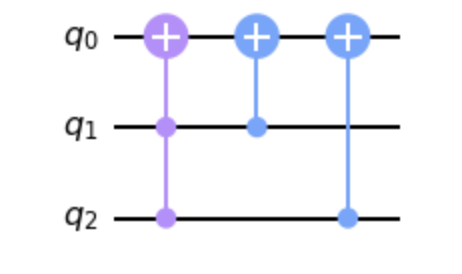
\includegraphics[scale=0.7]{reversibleOr.png}
\end{center}

\noindent This implementation was manually produced using a standard synthesis algorithm for reversible
circuits~\cite{10.1145/775832.775915}. To gain some intuition, we trace the evaluation of the circuit for input
\verb|011|. In this context, the most significant bit is at index 0. Thus the first \verb|ccx| gate negates \verb|q[0]|
since both \verb|q[1]| and \verb|q[2]| are true producing \verb|111|; the following \verb|cx| gate produces \verb|011|; finally the last \verb|cx| produces the result \verb|111|.

There is wealth of manual and algorithmic approaches for such synthesis problems each optimizing along  different dimensions~\cite{maslov:2003:rls:1087512,1201583}. Here is the circuit produced using an approach that analyzes the recursive structure of the circuit (and would generalise to computing the disjunction of more than two inputs):

\begin{center}
  \begin{minipage}[c]{0.4\linewidth}
\begin{verbatim}
reversibleOr2.qasm:

  // setup
  cx  q[1], q[0];
  x   q[1];
  ccx q[1], q[2], q[0];
  x   q[1];
  // measure
  \end{verbatim}
  \end{minipage}
  \qquad
  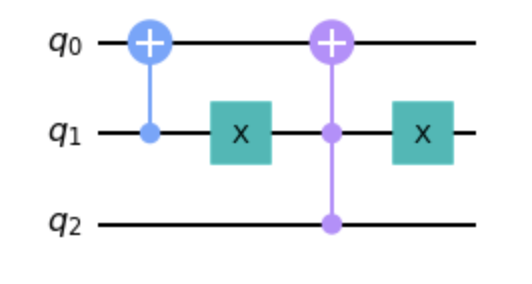
\includegraphics[scale=0.7]{reversibleOr2.png}
\end{center}

\noindent The evaluation of this circuit prints the same truth table as above confirming their equivalence. Tracing the
evaluation on the same input value \verb|011| goes through the stages \verb|111|, \verb|101|, \verb|101|, and finally \verb|111|.

The situation for Shor's algorithm is just as described above but with a more involved function of the form $f(r) = a^{r} \mod N$ for fixed $a$ and $N$. The specification of the circuit is relatively straightforward to calculate. Here it is for $a=11$ and $N=15$:
\[\begin{array}{rcll}
g(r,h) &=& \left\{ \begin{array}{ll}
                     (r,h+1) & \mbox{when~$r$~even~and~$h$~even} \\
                     (r,h-1) & \mbox{when~$r$~even~and~$h$~odd} \\
                     (r,11-h) & \mbox{when~$r$~odd~and~$4 > h \geq 0$~or~$12 > h \geq 8$} \\
                     (r,19-h) & \mbox{when~$r$~odd~and~$8 > h \geq 4$~or~$16 > h \geq 12$}
                                \end{array}\right.
\end{array}\]

\noindent However, as explained in standard accounts of the algorithm (e.g., the Qiskit implementation), producing an efficient
modular exponentiation circuit from this specification  is not straightforward and is actually the bottleneck in Shor’s algorithm. Typical
derivations of the circuit start from elementary gates, build a circuit for reversible disjunction and conjunction of
booleans, a circuit for a half-adder, a circuit for computing the carry, progressing to a circuit for modular addition,
which is used to build a circuit for modular multiplication, and then finally a circuit for modular exponentiation
taking care at each step to avoid the exponential blowup (e.g., by implementing exponentiation by squaring instead of repeated
multiplication)~\cite{shorefficient}.

% \paragraph*{Our Technical Results.} The main result of the paper is a proof, formalized in the HoTT-Agda library, that
% the category of finite sets and bijections is the free rig groupoid; its structure is illustrated diagrammatically below:

% \[\begin{tikzcd}
%     \PiLang && \PiPlusLang && \PiHatLang && \UFin
%     \arrow["\evalt", from=1-1, to=1-3]
%     \arrow["\evalp", curve={height=-24pt}, from=1-3, to=1-5]
%     \arrow["\evalh", curve={height=-24pt}, from=1-5, to=1-7]
%     \arrow["\quotep", curve={height=-24pt}, from=1-5, to=1-3]
%     \arrow["\quoteh", curve={height=-24pt}, from=1-7, to=1-5]
%   \end{tikzcd}\]

% \noindent The nodes $\PiLang$, $\PiPlusLang$, and $\PiHatLang$ in the diagram each represent a syntactic weak 2-category
% (groupoid actually as all morphisms are isomorphisms) where the 0-cells represent types, the 1-cells represent
% reversible circuits, and the 2-cells represent circuit equivalences. In $\PiLang$, the circuits represent arbitrary
% permutations among finite sets with products and coproducts; in $\PiPlusLang$, the circuits represent arbitrary
% permutations among finite sets with only coproducts; and in $\PiHatLang$, the permutations are expressed using adjacent
% transpositions.

% The syntactic groupoid $\PiPlusLang$ is the free rig groupoid; $\UFin$ is the groupoid of finite sets and bijections
% represented as the \emph{univalent subuniverse of all finite types}. The $\evalp/\quotep$ and $\evalh/\quoteh$ arrows
% establish a \emph{symmetric monoidal biequivalence} between these two groupoids. To get a taste of the involved
% complexity of this result, consider the obvious fact that, semantically, i.e., in $\UFin$, there is only one bijection
% from the empty set to itself. However, in the free groupoid, there are an infinite number of isomorphisms from the empty
% type to itself that go through arbitrary complex subtypes, e.g., letting $\isoone$ be the type constructor for type
% isomorphisms we can have a sequence of syntactic equivalences
% $\zerot \isoone \zerot \times A \isoone \zerot \times (A + \zerot) \isoone (\zerot \times A) + (\zerot \times \zerot)
% \isoone (\zerot \times \zerot) + (\zerot \times A) \isoone \zerot + (\zerot \times A) \isoone \zerot + \zerot \isoone
% \zerot$, and all such isomorphisms must be identified using appropriate coherence laws. The technical device to achieve
% this normalization is as follows. First, we observe that 1-paths in $\UFin$ are permutations on finite sets with a fixed
% cardinality $n$, given by $\Aut[\Fin[n]]$, which produce the permutation group on $\Fin[n]$, or the symmetric group
% $\Sn$. By giving a presentation of $\Sn$ using generators and relations, we build a rewriting system using the Coxeter
% relations~\cite{XXX} on the set of words $\List[\Fin[n]]$, and show that it is (locally) confluent and strongly
% normalizing. We then establish that the symmetric group $\Sn$ is the set-quotient of $\List[\Fin[n]]$ by the Coxeter
% relations, and show that it produces a group presentation, as a quotient of the free group. Using this strongly
% normalizing rewriting system, we establish that normal forms for words in $\Sn$ are Lehmer
% codes~\cite{lehmerTeachingCombinatorialTricks1960}, which are a convenient and compact representation of
% permutations. Finally, we show that there is an equivalence between Lehmer codes and permutations $\Aut[\Fin[n]]$ given
% by the Lehmer encode-decode algorithm.

% Below we reduce $\mathsf{swap} : 2 + 2 \leftrightarrow 2 + 2$ to a sequence of adjacent swaps. This is an example of
% a translation from $\PiPlusLang$ to $\PiHatLang$.

% \begin{align*}
%   \begin{tikzpicture}[scale=0.4,every node/.style={scale=0.4}]
%     \begin{knot}[clip width=3]
%       \filldraw (0,4) circle (2pt) node[above] {0};
%       \filldraw (1,4) circle (2pt) node[above] {1};
%       \filldraw (2,4) circle (2pt) node[above] {2};
%       \filldraw (3,4) circle (2pt) node[above] {3};
%       \filldraw (0,0) circle (2pt) node[below] {2};
%       \filldraw (1,0) circle (2pt) node[below] {3};
%       \filldraw (2,0) circle (2pt) node[below] {0};
%       \filldraw (3,0) circle (2pt) node[below] {1};
%       \strand (0,4) .. controls (0.5,1.5) and (1.5,2.5) .. (2,0);
%       \strand (1,4) .. controls (1.5,1.5) and (2.5,2.5) .. (3,0);
%       \strand (2,4) .. controls (1.5,1.5) and (1.5,2.5) .. (0,0);
%       \strand (3,4) .. controls (2.5,1.5) and (2.5,2.5) .. (1,0);
%     \end{knot}
%   \end{tikzpicture}
% \quad=\quad
%   \begin{tikzpicture}[scale=0.4,every node/.style={scale=0.4}]
%     \begin{knot}[clip width=3]
%       \filldraw (0,4) circle (2pt) node[above] {0};
%       \filldraw (1,4) circle (2pt) node[above] {1};
%       \filldraw (2,4) circle (2pt) node[above] {2};
%       \filldraw (3,4) circle (2pt) node[above] {3};
%       \filldraw (0,0) circle (2pt) node[below] {0};
%       \filldraw (1,0) circle (2pt) node[below] {2};
%       \filldraw (2,0) circle (2pt) node[below] {1};
%       \filldraw (3,0) circle (2pt) node[below] {3};
%       \strand (0,4) to (0,0);
%       \strand (1,4) .. controls (0.5,2) and (2.5,2) .. (2,0);
%       \strand (2,4) .. controls (2.5,2) and (0.5,2) .. (1,0);
%       \strand (3,4) to (3,0);
%     \end{knot}
%   \end{tikzpicture}
%   &&
%     \begin{tikzpicture}[scale=0.4,every node/.style={scale=0.4}]
%       \begin{knot}[clip width=3]
%         \filldraw (0,4) circle (2pt) node[above] {0};
%         \filldraw (1,4) circle (2pt) node[above] {2};
%         \filldraw (2,4) circle (2pt) node[above] {1};
%         \filldraw (3,4) circle (2pt) node[above] {3};
%         \filldraw (0,0) circle (2pt) node[below] {2};
%         \filldraw (1,0) circle (2pt) node[below] {0};
%         \filldraw (2,0) circle (2pt) node[below] {1};
%         \filldraw (3,0) circle (2pt) node[below] {3};
%         \strand (0,4) .. controls (-0.5,2) and (1.5,2) .. (1,0);
%         \strand (1,4) .. controls (1.5,2) and (-0.5,2) .. (0,0);
%         \strand (2,4) to (2,0);
%         \strand (3,4) to (3,0);
%       \end{knot}
%     \end{tikzpicture}
%   &&
%   \begin{tikzpicture}[scale=0.4,every node/.style={scale=0.4}]
%     \begin{knot}[clip width=3]
%       \filldraw (0,4) circle (2pt) node[above] {2};
%       \filldraw (1,4) circle (2pt) node[above] {0};
%       \filldraw (2,4) circle (2pt) node[above] {1};
%       \filldraw (3,4) circle (2pt) node[above] {3};
%       \filldraw (0,0) circle (2pt) node[below] {2};
%       \filldraw (1,0) circle (2pt) node[below] {0};
%       \filldraw (2,0) circle (2pt) node[below] {3};
%       \filldraw (3,0) circle (2pt) node[below] {1};
%       \strand (0,4) to (0,0);
%       \strand (1,4) to (1,0);
%       \strand (2,4) .. controls (1.5,2) and (3.5,2) .. (3,0);
%       \strand (3,4) .. controls (3.5,2) and (1.5,2) .. (2,0);
%     \end{knot}
%   \end{tikzpicture}
%   &&
%     \begin{tikzpicture}[scale=0.4,every node/.style={scale=0.4}]
%       \begin{knot}[clip width=3]
%         \filldraw (0,4) circle (2pt) node[above] {2};
%         \filldraw (1,4) circle (2pt) node[above] {0};
%         \filldraw (2,4) circle (2pt) node[above] {3};
%         \filldraw (3,4) circle (2pt) node[above] {1};
%         \filldraw (0,0) circle (2pt) node[below] {2};
%         \filldraw (1,0) circle (2pt) node[below] {3};
%         \filldraw (2,0) circle (2pt) node[below] {0};
%         \filldraw (3,0) circle (2pt) node[below] {1};
%         \strand (0,4) to (0,0);
%         \strand (1,4) .. controls (0.5,2) and (2.5,2) .. (2,0);
%         \strand (2,4) .. controls (2.5,2) and (0.5,2) .. (1,0);
%         \strand (3,4) to (3,0);
%       \end{knot}
%     \end{tikzpicture}
% \end{align*}

% \note{Show codes; normalize; explain the dense paragraph above using that example}

The technical result implies several immediate applications to reversible circuits: (i) a reversible circuit expressed
in $\PiPlusLang$ can be automatically generated from a permutation in $\UFin$ \emph{and the generation comes equipped
  with a proof of correctness establishing its equivalence between the circuit and the original permutation}; (ii)
circuits in $\PiLang$ or $\PiPlusLang$ can be reduced to a circuit normal form using a normalization by evaluation
process that evaluates them to a permutation in $\UFin$ and quotes it back; (iii) equivalence of circuits in either
$\PiLang$ or $\PiPlusLang$ can be decided by reducing them to normal forms; (i) a circuit can be verified against a
given permutation by evaluating it; and (v) the induced circuit equivalences in $\PiLang$ and $\PiPlusLang$ form a sound
and complete calculus for reasoning about and optimizing circuits. (See Sec.~\ref{sec:informal} for more details.)

  % \note{perhaps a note about the result being folklore; assumed in many places; but no proof; and certainly none
  %   formalized in a proof assistant. In some sense, what we have done is to take MacLane's coherence theorem and
  %   formalized it in HoTT, and given presentations for it using Pi's syntax. Also relevant is that the equivalence
  %   result hides implicit isomorphisms that have computational relevance. For example, transporting properties across
  %   equivalences of finite types can be done via executing permutations, something which has a clear computational cost
  %   and which itself depends on the choice of representations of the permutations.}

% \begin{itemize}[leftmargin=*]
%   \item We take the $\PiLang$ family of reversible languages~\cite{jamesInformationEffects2012} and show how to encode
%         various boolean reversible circuits in the language. The circuits are implemented using 1-combinators in the
%         language, and circuit optimisations are realized as 2-combinators between these reversible programs.
%   \item We show how to encode reversible circuits on a fixed number of bits as permutations of finite sets with the
%         appropriate cardinality. We observe that reversible programs can be translated to bijective functions between
%         finite sets and equality of reversible programs can be witnessed as extensional equality of these bijective
%         functions.
%   \item We review a few basics of Homotopy Type Theory~\cite{univalentfoundationsprogramHomotopyTypeTheory2013}, and
%         exhibit some results that we use in our technical development. We define the notion of a universe \`{a} la
%         Tarski internally in HoTT, which is given by a type for codes $U$ and a decoding function to a univalent
%         universe $\El : U \to \UU$. We say that this universe is univalent, if the decoding fibration is univalent, that
%         is, the decoding function $\El$ reflects the path space of the underlying univalent universe. We exhibit some
%         examples of univalent subuniverses, in particular, we define the subuniverse of finite types, $\UFin$, which
%         classifies all finite types, and show that it is univalent. Using this, we establish a characterization of the
%         path space of the universe of finite types.
%   \item We observe that 1-paths in $\UFin$ are permutations on finite sets with a fixed cardinality $n$, given by
%         $\Aut[\Fin[n]]$, which produces the permutation group on $\Fin[n]$, or the symmetric group $\Sn$. We then
%         proceed to give a presentation of $\Sn$ using generators and relations, by defining the Coxeter relations. We
%         build a rewriting system using the Coxeter relations on the set of words $\List[\Fin[n]]$, and show that it is
%         (locally) confluent and strongly normalising. We define the the symmetric group $\Sn$ to be the set-quotient of
%         $\List[\Fin[n]]$ by the Coxeter relations, and show that it produces a group presentation, as a quotient of the
%         free group. Using our strongly normalising rewriting system, we establish that normal forms for words in $\Sn$
%         are Lehmer codes~\cite{lehmerTeachingCombinatorialTricks1960}, which are a convenient and compact representation
%         of permutations for permutations. Finally, we show that there is an equivalence between Lehmer codes and
%         permutations $\Aut[\Fin[n]]$ given by the Lehmer encode-decode algorithm.
%   \item Finally, we show how to interpret the language $\PiLang$ into our groupoid $\UFin$, in stages. First we define a
%         subset of the language $\PiPlusLang$ which only includes the additive monoidal structure. We translate $\PiLang$
%         programs to $\PiPlusLang$ by defining multiplication as repeated addition. Then, we further define a normalized
%         form for for this language called $\PiHatLang$, which has normalized 1-combinators and 2-combinators
%         corresponding to adjacent transpositions. We show that $\PiPlusLang$ can be translated to $\PiHatLang$ and back,
%         using adjacent transpositions to generate arbitrary swaps. Then, we show how to interpret this language
%         $\PiHatLang$ into $\UFin$ -- the 1-combinators are translated into permutations via words in $\Sn$, and
%         2-combinators are interpreted as 2-paths in $\UFin$. We further show how to quote back a permutation in $\UFin$
%         into a 1-combinator using the normal form for words in $\Sn$.
%   \item We give some applications of this translation by showing how to normalise a circuit written in $\PiLang$ to a
%         normal form in $\PiPlusLang$ and $\PiHatLang$, which uses fewer gates.~\todo{Here, or earlier?}
% \end{itemize}

% Our results are formalized in the proof assistant Agda using the HoTT-Agda library.

% \begin{center}
%   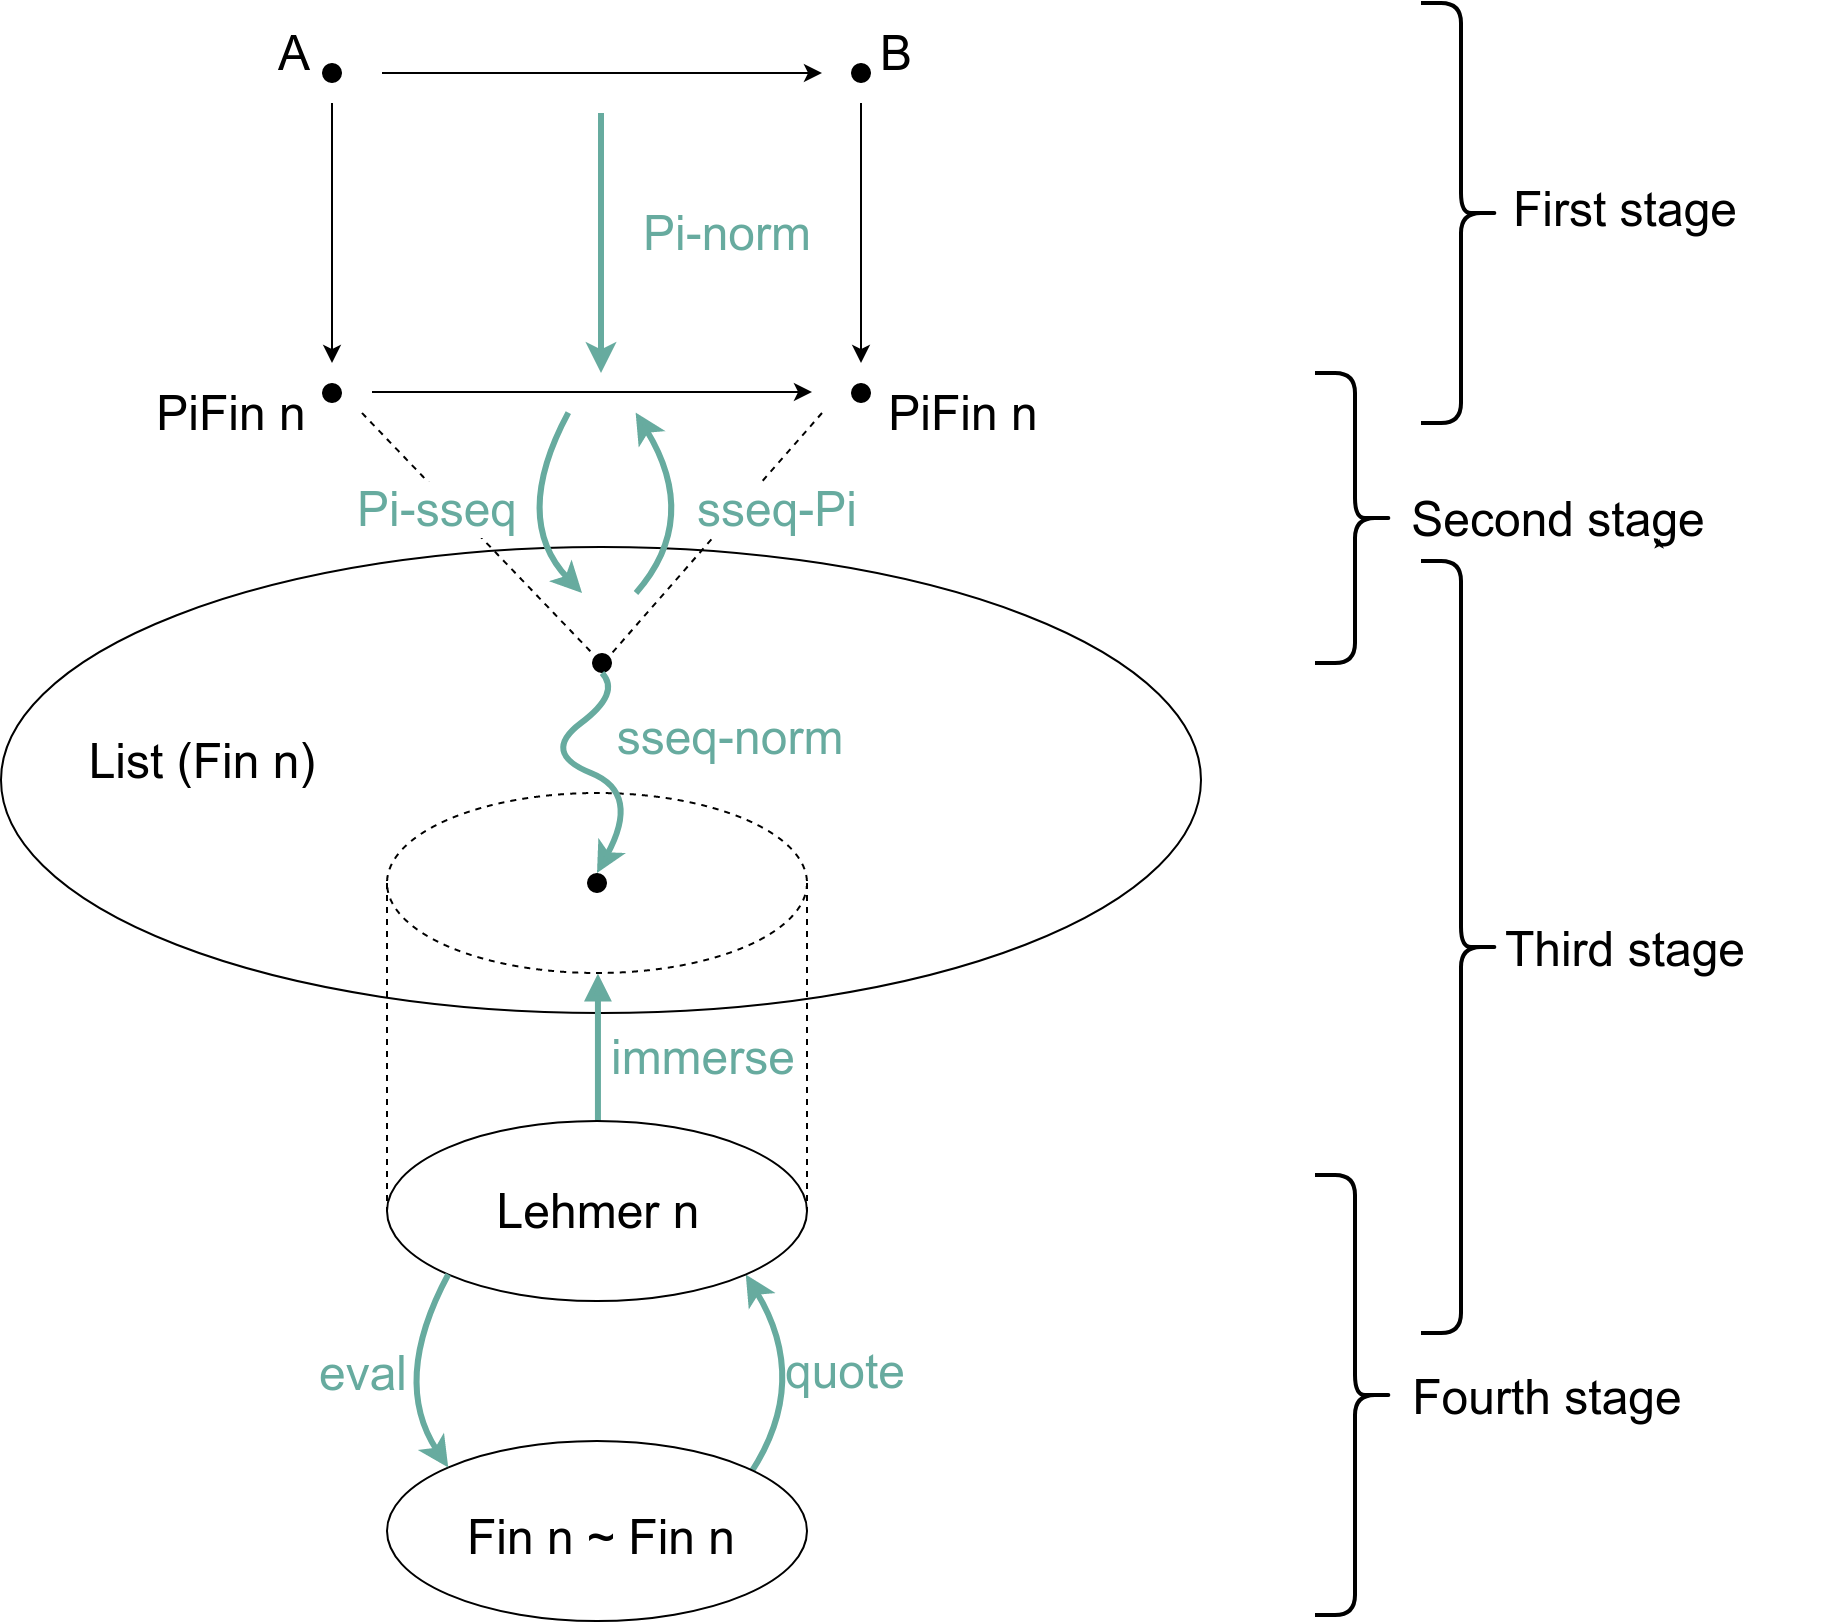
\includegraphics[scale=0.3]{outline.png}
% \end{center}

% \note{Redo this figure or delete ??}

%% \note{Spiel about reversible computing and logical reversibility ??}

%% \note{Spiel about using groupoids for denotational semantics ??}

%% \note{Could we include a short paragraph about entropy and bits and logical reversibility ??}

%% \note{Novel interpretation of the univalence axiom, operational and denotational semantics and adequacy.}

% * STLC(first) is the type theory for CCC
%   HoTT is type theory for weak infty groupoids(first)
%   Correspondence between TT and categories are fruitful:
%   answer hard questions about syntax without worrying about presentation
%   normalization of lcal with strong sums: if you have specific syntax; no obvious induction on syntax
%   Lawvere thesis


% * Rig groupoids are interesting! WHY????
%   Add monoidal structure to weak groupoids. Easy. Lists
%   How symmetry is going to act on higher dimension
%   Higher-dim all symmetric; topology higher things abelian groups

% * What is the corresponding type theory ?
%   We give it for the free symmetric groupoid; for other groupoids build on it and add more




%%% Local Variables:
%%% mode: latex
%%% TeX-master: "main"
%%% fill-column: 120
%%% End:

\note{Things that were in extra that should be integrated}

\begin{verbatim}
Combinators in the (List 3) are acting on << 4 >>
so

(1 :: 2 :: 0 :: 1 :: nil) of type List 3

corresponds to the sequence:

swap 1 2 ;
swap 2 3 ;
swap 0 1;
swap 1 2

and swap 1 2 is then
   A + (B + (C + (D + 0)) <—> A + (C + (B + (D + 0))

also, swap 2 3 is
   A + (B + (C + (D + 0))) <—> A + (B + (D + (C + 0)))
\end{verbatim}

Although the meaning of a permutation - that is, the specific bijective function
that it represents - is in some sense all there is, manipulating them
syntactically still has its advantages. By writing reversible programs, we think
of them in an intensional way. Comparing two programs for equality by evaluating
them on all points in the domain is a very crude - and maybe even inefficient -
way of doing that. ~\cite{Kuehlmann:2006:RBR:2298470.2300327,10.1007/978-3-540-24605-3_4,Yamashita:2010:FEQ:1835957.1835965}.

It is crude, because there is no way of enforcing additional constraints on the
process of transforming one program into another, and no way of inspecting what
transformation occurred. We can imagine a practical situation in which reversible
circuits admit one kind of optimization \jk{FPGA?}, but do not admit another,
even though they are equivalent in the extensional sense - or maybe one of these
transformations is cheaper than another, or maybe it is important to know which
transformation did occur for the \jk{producer(?)} to focus their resources of
improving this kind of transformations. By comparing the circuits extensionally,
the proof object = the path from one into the other - does not have any
structure,  it is just a check that the values match.

On the other hand, even though in general, the equality of circuits requires
exponential time jk{triple check}, the proof object can be still very small.
This creates structure that can possibly be exploited in a heuristic way.
\jk{Additionally, if the goal is to convince third-party that two circuits are
the same, we can just present the proof instead of showing the equality directly
- for example, by choosing a particularly short one}.

Taking all this into account, it is clear that we must seek a syntactic way of
computing the meaning of the circuit, instead of just directly evaluating it to
$\Aut[\Fin[n]]$ - since when we go back and quote the permutation as a circuit
(in a normal form), there was no "trace" left to see what transformation (what
sequence of 2-paths) maps the old one into the new one.

We are additionally experimenting with user annotations that can guide
the search. Each level-2 combinator can be annotated with various
``cost'' annotations indicating whether it reduces the number of
gates, reduces the number of choice points, or other cost
functions. Then one can ask for a proof that takes no more than a
certain number of steps or a proof that does not create more than a
certain number of additional wires etc. We illustrate these ideas by
defining a simple cost function and using it to annotate level-2
combinators.

We define the \emph{length} $L(c)$ of a composite circuit $c$ as
follows: the length of a sequential composition of circuits is the sum
of the lengths of the subcircuits $L(f \odot g) = L(f) + L(g)$; and
the length of choice or parallel composition is the maximum of either
branch $L(f \oplus g) = L(f \otimes g) = \max(L(f),L(g))$. For
primitive gates, the length needs to be postulated to reflect the
``length'' of the computation involved in applying that primitive. As
examples, consider the following two level-2 combinators:

% \begin{code}
% linv◎l'  :  {t₁ t₂ : U} {c : t₁ ⟷ t₂} → (c ◎ ! c) ⇔ id⟷
% idl◎l'   :  {t₁ t₂ : U} {c : t₁ ⟷ t₂} → (id⟷ ◎ c) ⇔ c
% \end{code}
% \AgdaHide{
% \begin{code}
% linv◎l'  = ?
% idl◎l'   = ?
% \end{code}
% }

\noindent Assuming that $\idc$ takes a unit length of computation, the
first can be annotated with $L(c)*2 \isotwo 1$ and the second with $L(c)+1 \isotwo
L(c)$ indicating that the first combinator reduces the length of the
circuit from twice the length of $c$ to 1 and the second combinator
reduces the length of the circuit by 1. Such annotations can then be
used to constrain or guide the search for transformations between
circuits.

we can transfer theorems about permutations from one representation to another


Natural numbers under addition form the free commutative monoid on one generator. Categorifying this, we get the free
symmetric monoidal groupoid on generators. This is the groupoid of finite sets and bijections.

More generally, we can construct the free symmetric monoidal groupoid on a groupoid, by taking the action of the
groupoid of finite sets and bijections. We can construct this in HoTT by using the classifying space of the symmetric
group.

The free symmetric monoidal category on a category is a 2-monad on
Cat~\cite{blackwellTwodimensionalMonadTheory1989,abramskyAbstractScalarsLoops2005,leinsterHigherOperadsHigher2004}.
Other applications are Fock Spaces, Generalised Species, Abstract Syntax.

We establish a Curry-Howard-Lambek correspondence for Pi, with 0, 1, +. Categorically, the syntactic groupoid of Pi is
the free symmetric monoidal groupoid on one generator. The groupoid of finite sets and bijections, with coproducts, is
equivalent to the free symmetric monoidal groupoid on one generator, making Pi fully adequate with respect to this
semantics.

The logic part of this is in superstructural reversible logic, which is the free commutative semirig, since there are no
equations.

perhaps fig. on p.30 of 4 different ways of going from a + (b + c) to c + (b + a) ??

Outline: of main paper; appendix for background on HoTT; for long proofs; etc. accompanying artifact

go through mails about paper

update popl sub

I pushed some new changes and merged to master.
The most interesting thing: a proof of the base case, which we have been fighting with for quite long. (it's in Equiv2Hat.agda)

% c₊⟷₂id⟷₁ : (c : O ⟷₁ O) → c ⟷₂ id⟷₁
% c₊⟷₂id⟷₁ c =
%         let x = quote^₂ (eval^₂-O c)
%         in  ((idr◎r ■ idl◎r) ■ !⟷₂ (quote-eval^₁ c)) ■ x
